\chapter{AMD64 ARCHITECTURE OVERVIEW}
\label{chap:amd64}
Typically a SoC brings together functionality that used to be distributed across chips or maybe even devices. Various functional modules of the system are integrated into a single chip set. Naturally SoCs are very complex designs which includes programming elements, hardware elements, software elements, bus architecture, clock and power distribution, test structures etc. 

The heart of any SoC design is a core which is nothing but some sort of processor, and practically all SoC is likely to have at least one processor. In AMD, most processors are based on AMD64 architecture. Majority of the verification scenarios are developed in reference to the behavior of core and hence makes it an important design of interest.

\section {AMD64 ARCHITECTURE}
The AMD64, originally called x86-64, architecture is a 64-bit, backward compatible extension of industry-standard x86 architecture (legacy)\cite{SS:AMD64-V1}. It adds 64-bit addressing and expands register resources to support higher performance for recompiled 64-bit programs, while supporting legacy 16-bit and 32-bit applications and operating systems without modification or recompilation. The need for a 64 bit x86 architecture is driven by applications that address large amounts of virtual and physical memory, such as high-performance servers, database management systems, and CAD tools. These applications benefit from both 64-bit addresses and an increased number of registers.



\section {FEATURES OF AMD64}
\addtocontents{toc}{\protect\setcounter{tocdepth}{1}}
The main features of AMD64 architecture are its extended 64-bit registers and new 64-bit mode of operation.  
\subsection{REGISTERS}

One of the main features of AMD64 architecture is the 64-bit register extension. The small number of registers available in the legacy x86 architecture limits performance in computation-intensive applications. Increasing the number of registers provides a performance boost to many such applications. In addition to the 8 legacy x86 General-Purpose Registers (GPRs), AMD64 introduce additional 8 GPRs. All 16 GPRs are 64-bit long and an instruction prefix (REX) accesses the extended registers. The architecture also introduces 8 new 128-bit media registers.
%\figurename{} 
\begin{figure}[h!]
\centering
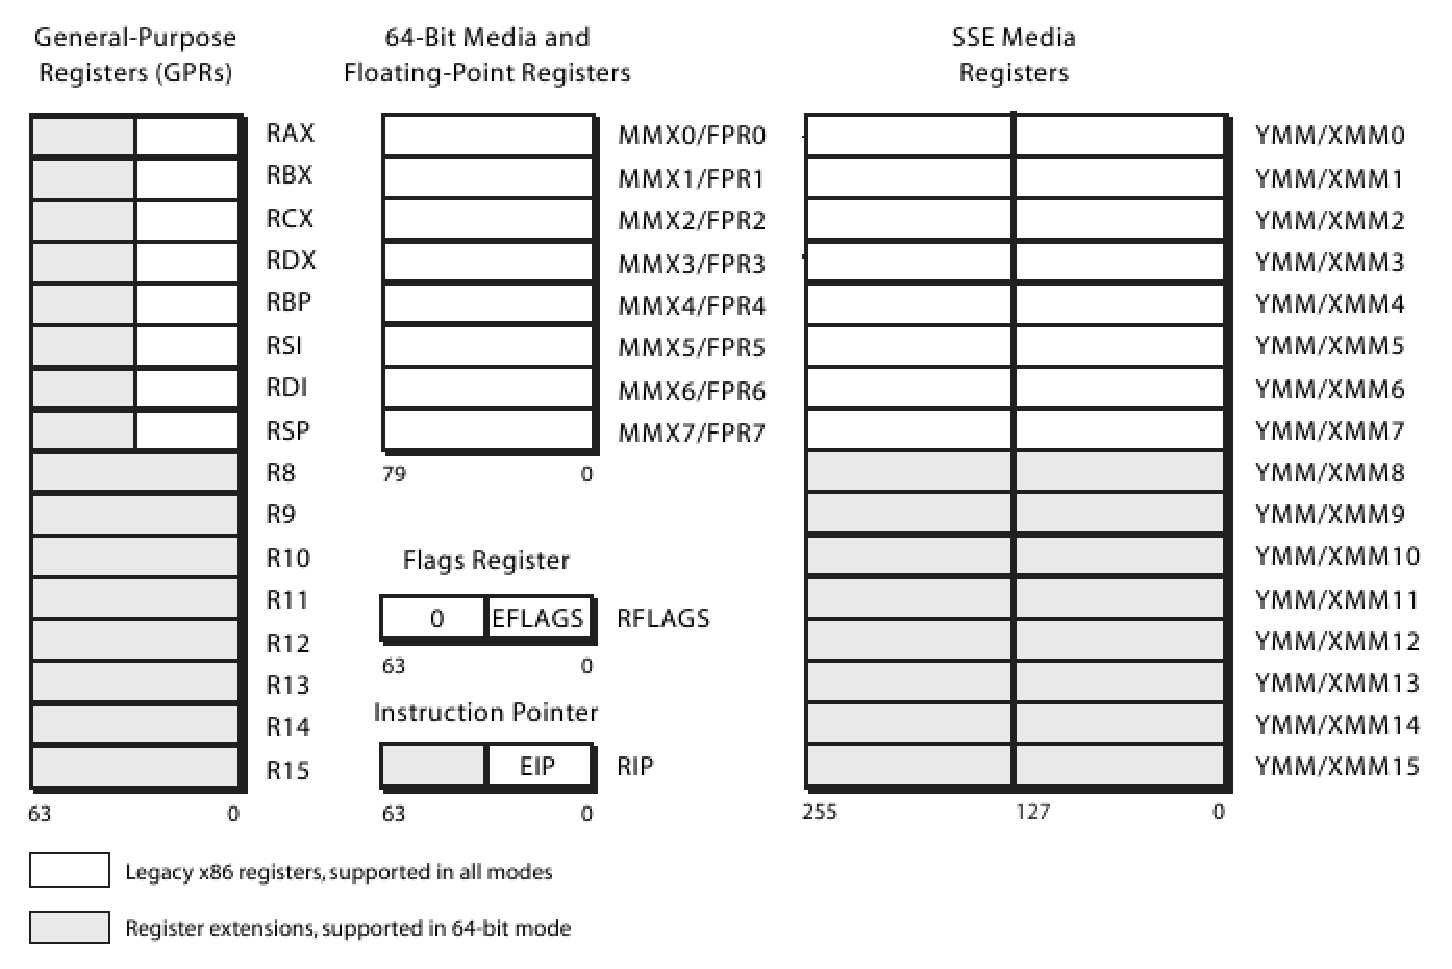
\includegraphics[scale=0.65]{./figures/registers.eps}
\caption{AMD64 Registers}
\label{fig:registers.eps}
\end{figure}


~\figurename{~\ref{fig:registers.eps}} shows the AMD64 application-programming register set. They include the general-purpose registers (GPRs), segment registers, flags register (64-bits), instruction-pointer register (64-bits) and the media registers. 

\subsection{MODES OF OPERATION}
In addition to the x86 legacy mode, another major feature of AMD64 for is its long mode. This is the mode where a 64-bit application (or operating system) can access 64-bit instructions and registers.%~\figurename{~\ref{fig:modes.eps}} shows the features of each mode of operation in AMD64 architecture. 
The different modes of operations in AMD64 architecture are detailed below:
%\begin{tabular}
%\figurename{} 
%\begin{figure}[h!]

%\centering
%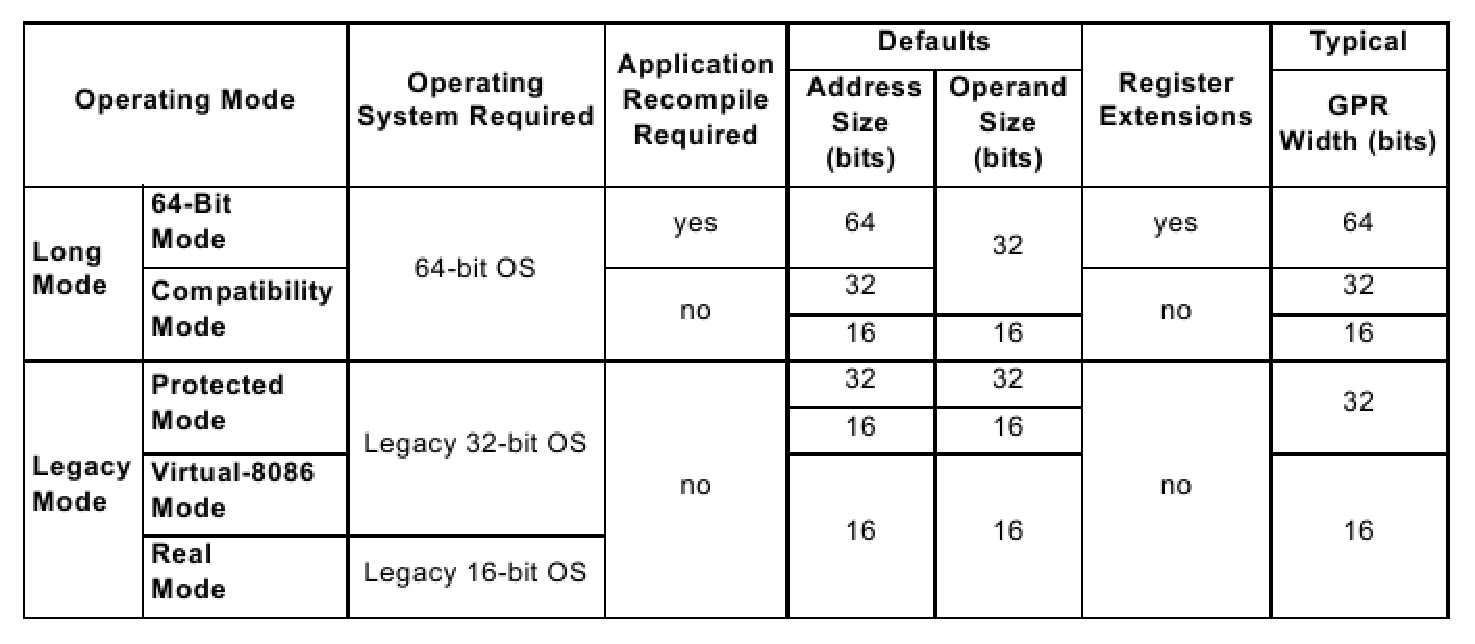
\includegraphics[width=6in]{./figures/modes.eps}
%\caption{AMD64 Modes of Operation}
%\label{fig:modes.eps}
%\end{figure}
%\end{tabular}



\emph {\bf Long Mode}: Long mode is an extension of legacy protected mode. It consists of two sub modes: 64-bit mode and compatibility mode. 64-bit mode supports all of the new features and register extensions of the AMD64 architecture. Compatibility supports binary compatibility with existing 16-bit and 32-bit applications. Long mode does not support legacy real mode or legacy virtual-8086 mode, and it does not support hardware task switching.
\begin{itemize}

\item 64-bit mode: 64-bit mode supports the full range of 64-bit virtual-addressing and register-extension features. This mode is enabled by the operating system on an individual code segment basis. As 64-bit mode supports a 64-bit virtual-address space, it requires a 64-bit operating system and tool chain.


\item Compatibility Mode: Compatibility mode allows 64-bit operating systems to run existing 16-bit and 32-bit x86 applications. These legacy applications run in compatibility mode without recompilation. This mode is also enabled by operating system on an individual code segment bases as in 64 bit mode. However unlike 64-bit mode x86 segmentation function similar to legacy x86 architecture using 16-bit or 32-bit protected mode semantics.

\end{itemize}



\emph {\bf Legacy Mode}: Legacy mode has compatibility existing 16-bit and 32-bit operating systems in addition to compatibility with existing 16-bit and 32-bit application. Legacy mode has the following three submodes : 

\begin{itemize}

\item Protected Mode: Legacy protected mode supports 16-bit and 32-bit programs with memory segmentation, optional paging, and privilege-checking. Programs in this mode can access up to 4GB of memory space.


\item Virtual-8086 Mode: Virtual-8086 mode supports 16-bit real-mode programs running as tasks under protected mode. It uses a simple form of memory segmentation, optional paging, and limited protection-checking. Programs in virtual-8086 mode can access up to 1MB of memory space.


\item Real Mode: Real mode supports 16-bit programs using register-based memory segmentation. It does not support paging or protection-checking. Programs running in real mode can access up to 1MB of memory space.
\end{itemize}

\section{MEMORY ORGANIZATION}
\addtocontents{toc}{\protect\setcounter{tocdepth}{1}}

The AMD64 architecture organizes memory into virtual memory and physical memory\cite{SS:AMD64-V2}. Virtual memory and physical-memory spaces are usually different in size with virtual address space being much larger than physical-address memory.  System software relocates applications and data between physical memory and the system hard disk to make it appear that much more memory is available than really exist and then uses the hardware memory-management mechanisms to map the larger virtual-address space into the smaller physical-address space.

\subsection {VIRTUAL MEMORY}
Virtual memory consists of the entire address space available. It is a large linear address space that is translated to a smaller physical address space. Programs uses virtual address space to access locations within the virtual memory space. System software is responsible for managing the relocation of applications and data in virtual memory space using segment-memory management. System software is also responsible for mapping virtual memory to physical memory through the use of page translation.

The architecture supports different virtual-memory sizes using the following modes:
\begin{itemize}

\item[-] Protected Mode: Supports 4 gigabytes of virtual-address space using 32-bit virtual  addresses.

\item[-] Long Mode: Supports 16 exabytes of virtual-address space using 64-bit virtual addresses.
\end{itemize}

\subsection {PHYSICAL MEMORY}
Physical addresses are used to directly access main memory. This is the installed memory in a particular system that can be physically accessed by the bus interfaces. The larger virtual address space is translated to smaller physical address space through two translation stages called segmentation and paging. The architecture supports different physical-memory sizes using the following modes:
\begin{itemize}

\item[-] Real Mode- Supports 1 Megabyte of physical-address space using 20-bit physical addresses.

\item[-] Legacy Protected Mode- Supports several different address-space sizes, depending on the translation. supports 4 gigabytes of physical address space using 32-bit physical addresses and when the physical-address size extensions are enabled, the page-translation mechanism can be extended to support 52-bit physical addresses.

\item[-] Long Mode- Supports up to 4 petabytes of physical-address space using 52-bit physical addresses. Long mode requires the use of page-translation and the physical-address size extensions (PAE).

\end{itemize}






\section{MEMORY MANAGEMENT}

\addtocontents{toc}{\protect\setcounter{tocdepth}{1}}

Memory management refers to the process involved in translating address generated by software to physical address through segmentation and paging. This process is hidden from application software and is handled by system software and processor hardware. 


\subsection{SEGMENTATION} 
Segmentation mainly helps system software to isolate software processes (tasks) and the data used by that process to increase the reliability of system running multiple process simultaneously. The AMD64 architecture is designed to support all forms of legacy segmentation. In 64-bit mode segmentation is not adopted (use flat band segmentation) [AMD64]. Segmentation is, however, used in compatibility mode and legacy mode. 
~\figurename{~\ref{fig:segmentation.eps}}shows segmented virtual memory.

%\figurename{} 
\begin{figure}[H]
\centering
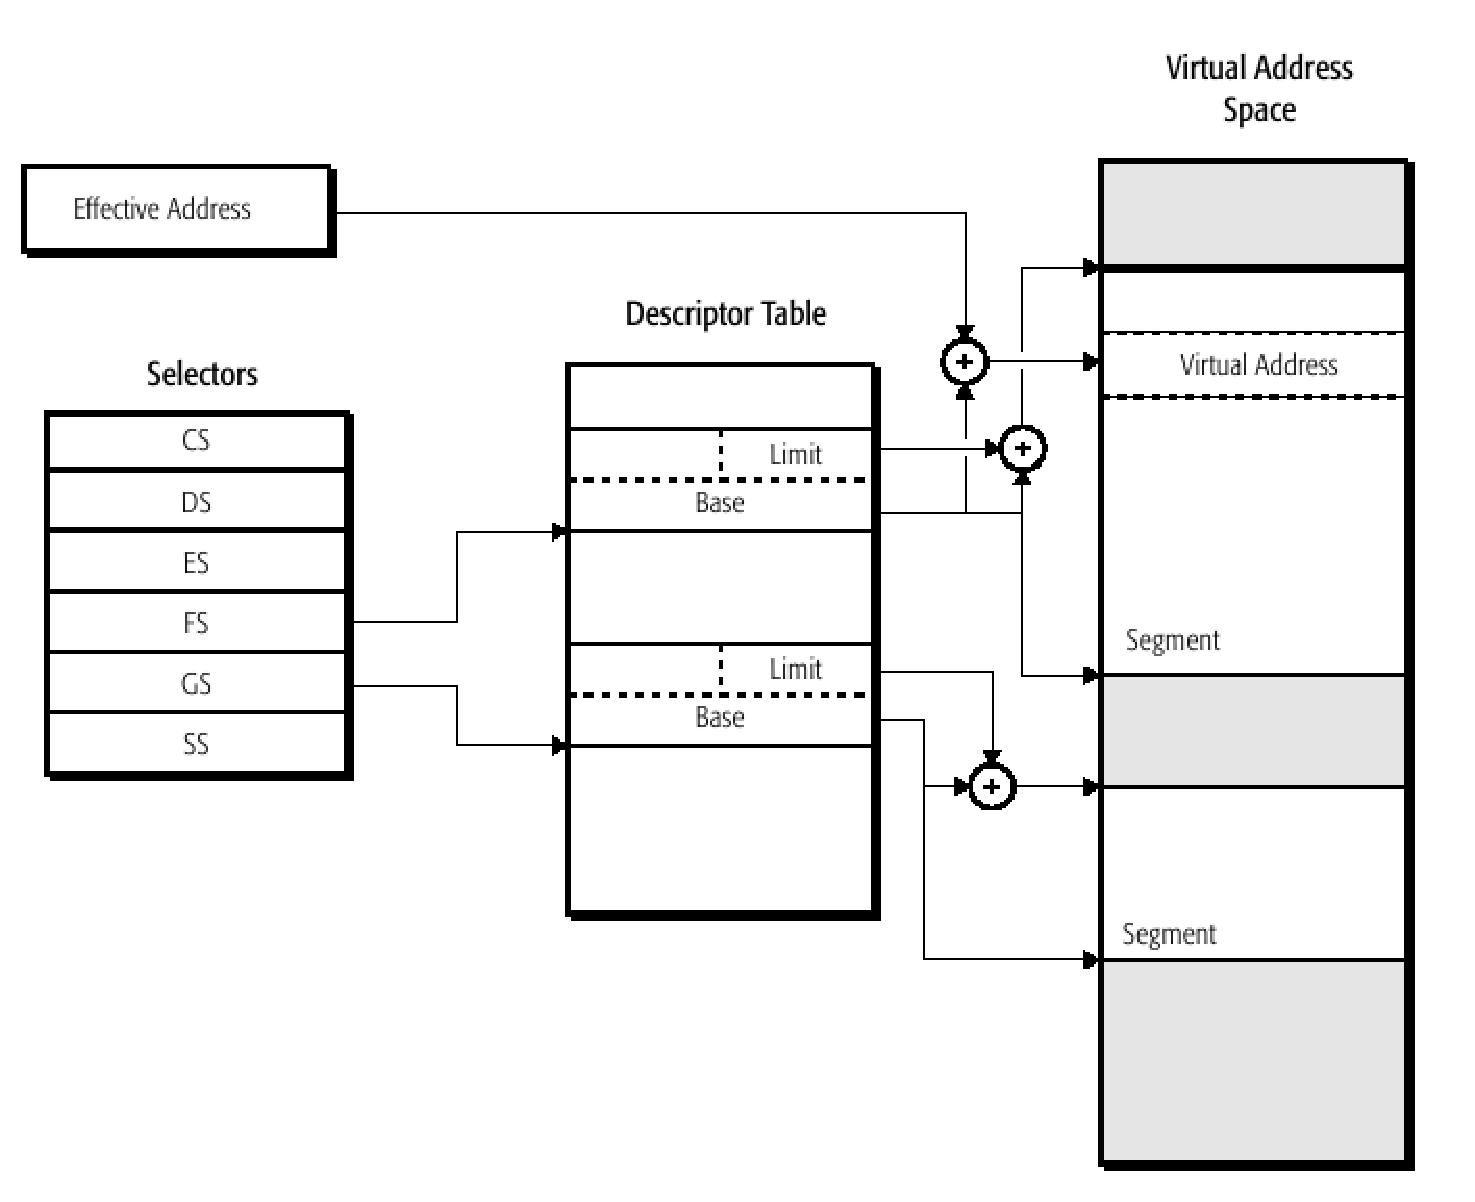
\includegraphics[scale=0.5]{./figures/segmentation.eps}
\caption{Segmented Memory Model}
\label{fig:segmentation.eps}
\end{figure}


The segmentation mechanism provides ten segment registers, each of which defines a single segment. Six of these registers (CS, DS, ES, FS, GS, and SS) define user segments. The remaining four segment registers (GDT, LDT, IDT, and TR) define system segments. The segment selector points toward a specific entry in descriptor table. This can be Global Descriptor Table (GDT) or Local Descriptor Table (LDT). The descriptor table entry base value plus the effective address which is the offset from base gives the virtual address. Effective address is calculated from the value stored in general purpose register and a displacement value encoded as part of instruction.

\subsection{PAGING}
Paging allows software and data to be relocated in physical address space using fixed-size blocks called physical pages. It translation uses a hierarchical data structure called a page-translation table to translate virtual pages into physical pages. Paging also provides protection as access to physical pages by lesser-privileged software can be restricted. ~\figurename{~\ref{fig:paging.eps}}shows an example of paged memory with three levels in the translation-table hierarchy. 




%\figurename{} 
\begin{figure}[H]
\centering
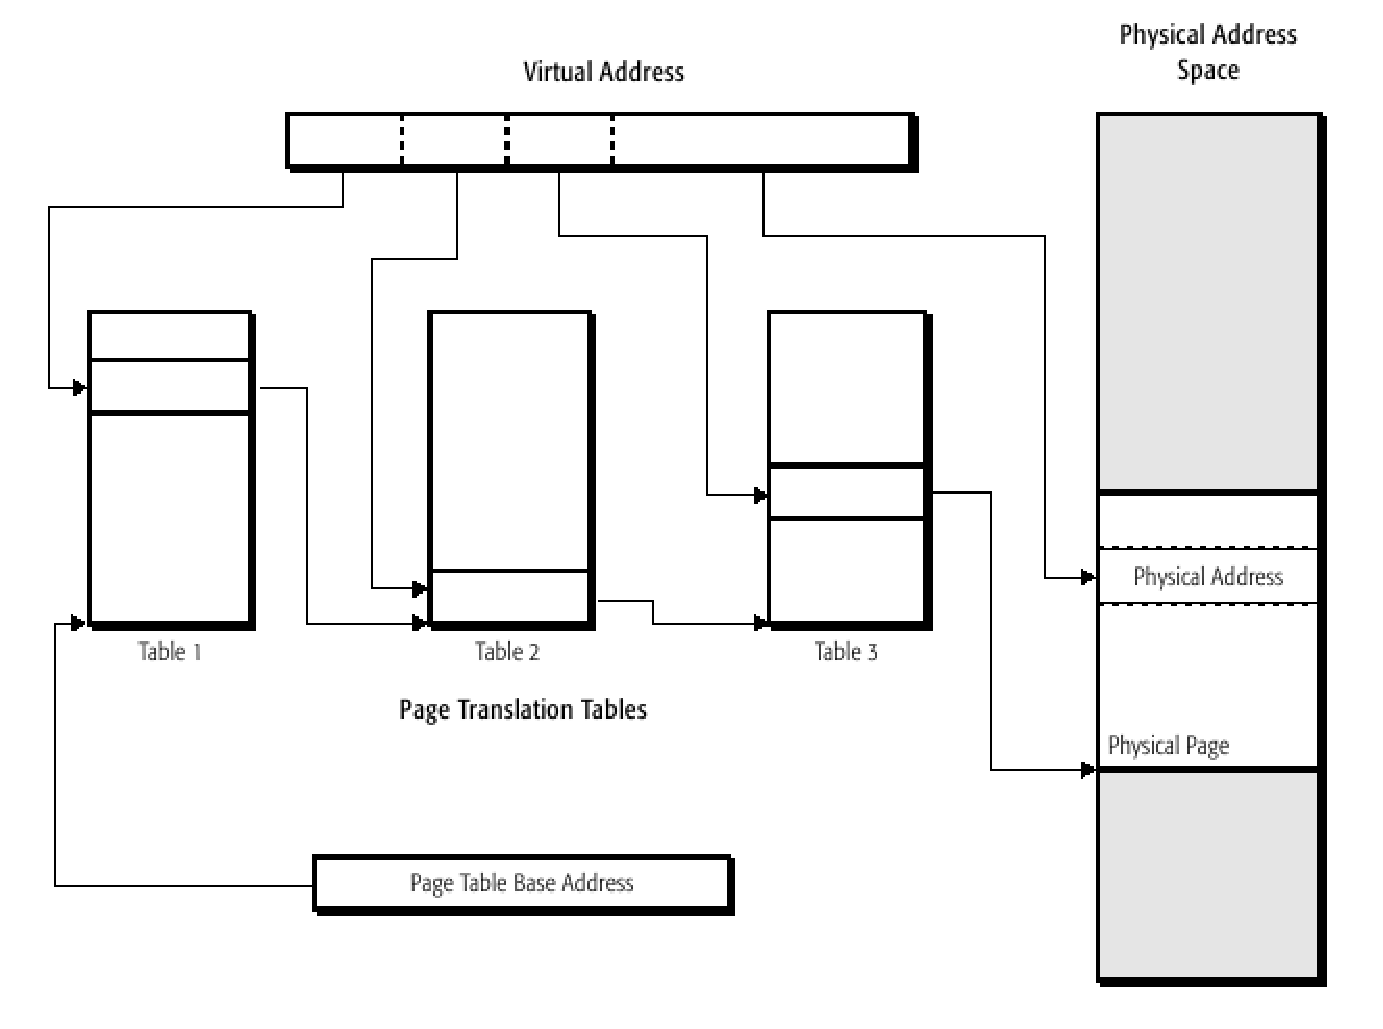
\includegraphics[scale=0.5]{./figures/paging.eps}
\caption{Paged Memory Model}
\label{fig:paging.eps}
\end{figure}



The number of levels in the translation-table hierarchy can be as few as one or as many as four, depending on the physical-page size and processor operating mode. Each table in the translation hierarchy is indexed by a portion of the virtual-address bits. The entry referenced by the table index contains a pointer to the base address of the next-lower level table in the translation hierarchy. Last page table entry plus the offset value from the virtual address (lsb bits), points toward the actual physical address.  

